\documentclass[aspectratio=169]{beamer}
\usepackage{lmodern}
\usetheme{Madrid}
%\usecolortheme{giantoak}
\newcommand*\oldmacro{}
\let\oldmacro\insertshorttitle
\renewcommand*\insertshorttitle{\oldmacro\hfill\insertframenumber\,/\,\inserttotalframenumber}
\usepackage[framemethod=tikz]{mdframed}

\usepackage{beamerthemesplit}
\usepackage{textpos}
\usepackage{pgf}
%\logo{\pgfputat{\pgfxy(0,-.4)}{\pgfbox[right,base]{\includegraphics[height=1.0cm]{logo.jpg}}}}
%\newcommand{\nologo}{\setbeamertemplate{logo}{}}
\usepackage{booktabs}
\usepackage{graphicx}
\theoremstyle{principle}
\newtheorem*{principle}{Design Principle}


\titlegraphic{\includegraphics[width=1.0\paperwidth]{cool-wind-800px.jpg}}

\title{Amendments}
%\author[Jeremy Kedziora]{Wind Data Science Team\\
%\small{Uptake}}
\date{}

\begin{document}

%{
%%\nologo
%\begin{frame}
%    \maketitle
%\end{frame}
%}
%pages 1-7, 8-9, 14-15.


{
  \usebackgroundtemplate{\includegraphics[width=1.0\paperwidth]{policy.png}}
  \begin{frame}[plain]
  
\begin{mdframed}[tikzsetting={draw=black,fill=white,fill opacity=0.7,
               line width=0pt},backgroundcolor=none,leftmargin=20,
               rightmargin=20,innertopmargin=4pt]
\Huge Stone
\end{mdframed}

  \end{frame}
}

%@@@@@@@@@@@@@@@@@@@@@@@@@@@@@@@@@@@@@@@@@@@@@@@@@
%\begin{frame}
%
%\begin{center}
%\includegraphics[scale=0.4]{lake_michigan.jpg}
%\end{center}
%
%
%\end{frame}



%@@@@@@@@@@@@@@@@@@@@@@@@@@@@@@@@@@@@@@@@@@@@@@@@@
\begin{frame}

\begin{center}
\Huge\textbf{Problems : Numbers}\\
\bigskip
\bigskip
\large Describing with numbers
\end{center}

\end{frame}

%%@@@@@@@@@@@@@@@@@@@@@@@@@@@@@@@@@@@@@@@@@@@@@@@@@
%\begin{frame}
%\frametitle{Choices}
%\begin{itemize}
%\item How do we measure unemployment?
%\begin{itemize}
%\item \textbf{Decide} what the measure is supposed to capture: need for jobs;
%\item \textbf{Transform} this into something observable: people wanting work;
%\item \textbf{Operationalize} by fixing inclusion criteria: older than 16, had a job previously, have looked in previous 4 weeks, and are available;
%\end{itemize}
%\bigskip
%\bigskip
%\item Definition of measurement $=$ definition of the problem and therefore a main avenue of political conflict;
%\bigskip
%\bigskip
%\item Stone wonders about those who...
%\begin{itemize}
%\item ...can get dangerous/demeaning/unpleasant jobs but don't;
%\item ...could get part time but hold out for full time;
%\item ...quit to find something better but are still searching;
%\item ...can get a job but can't find child care to take a job;
%\item ...have never worked but want to now.
%\end{itemize}
%
%\end{itemize}
%\end{frame}


%@@@@@@@@@@@@@@@@@@@@@@@@@@@@@@@@@@@@@@@@@@@@@@@@@
\begin{frame}
\frametitle{Choices}
\begin{center}
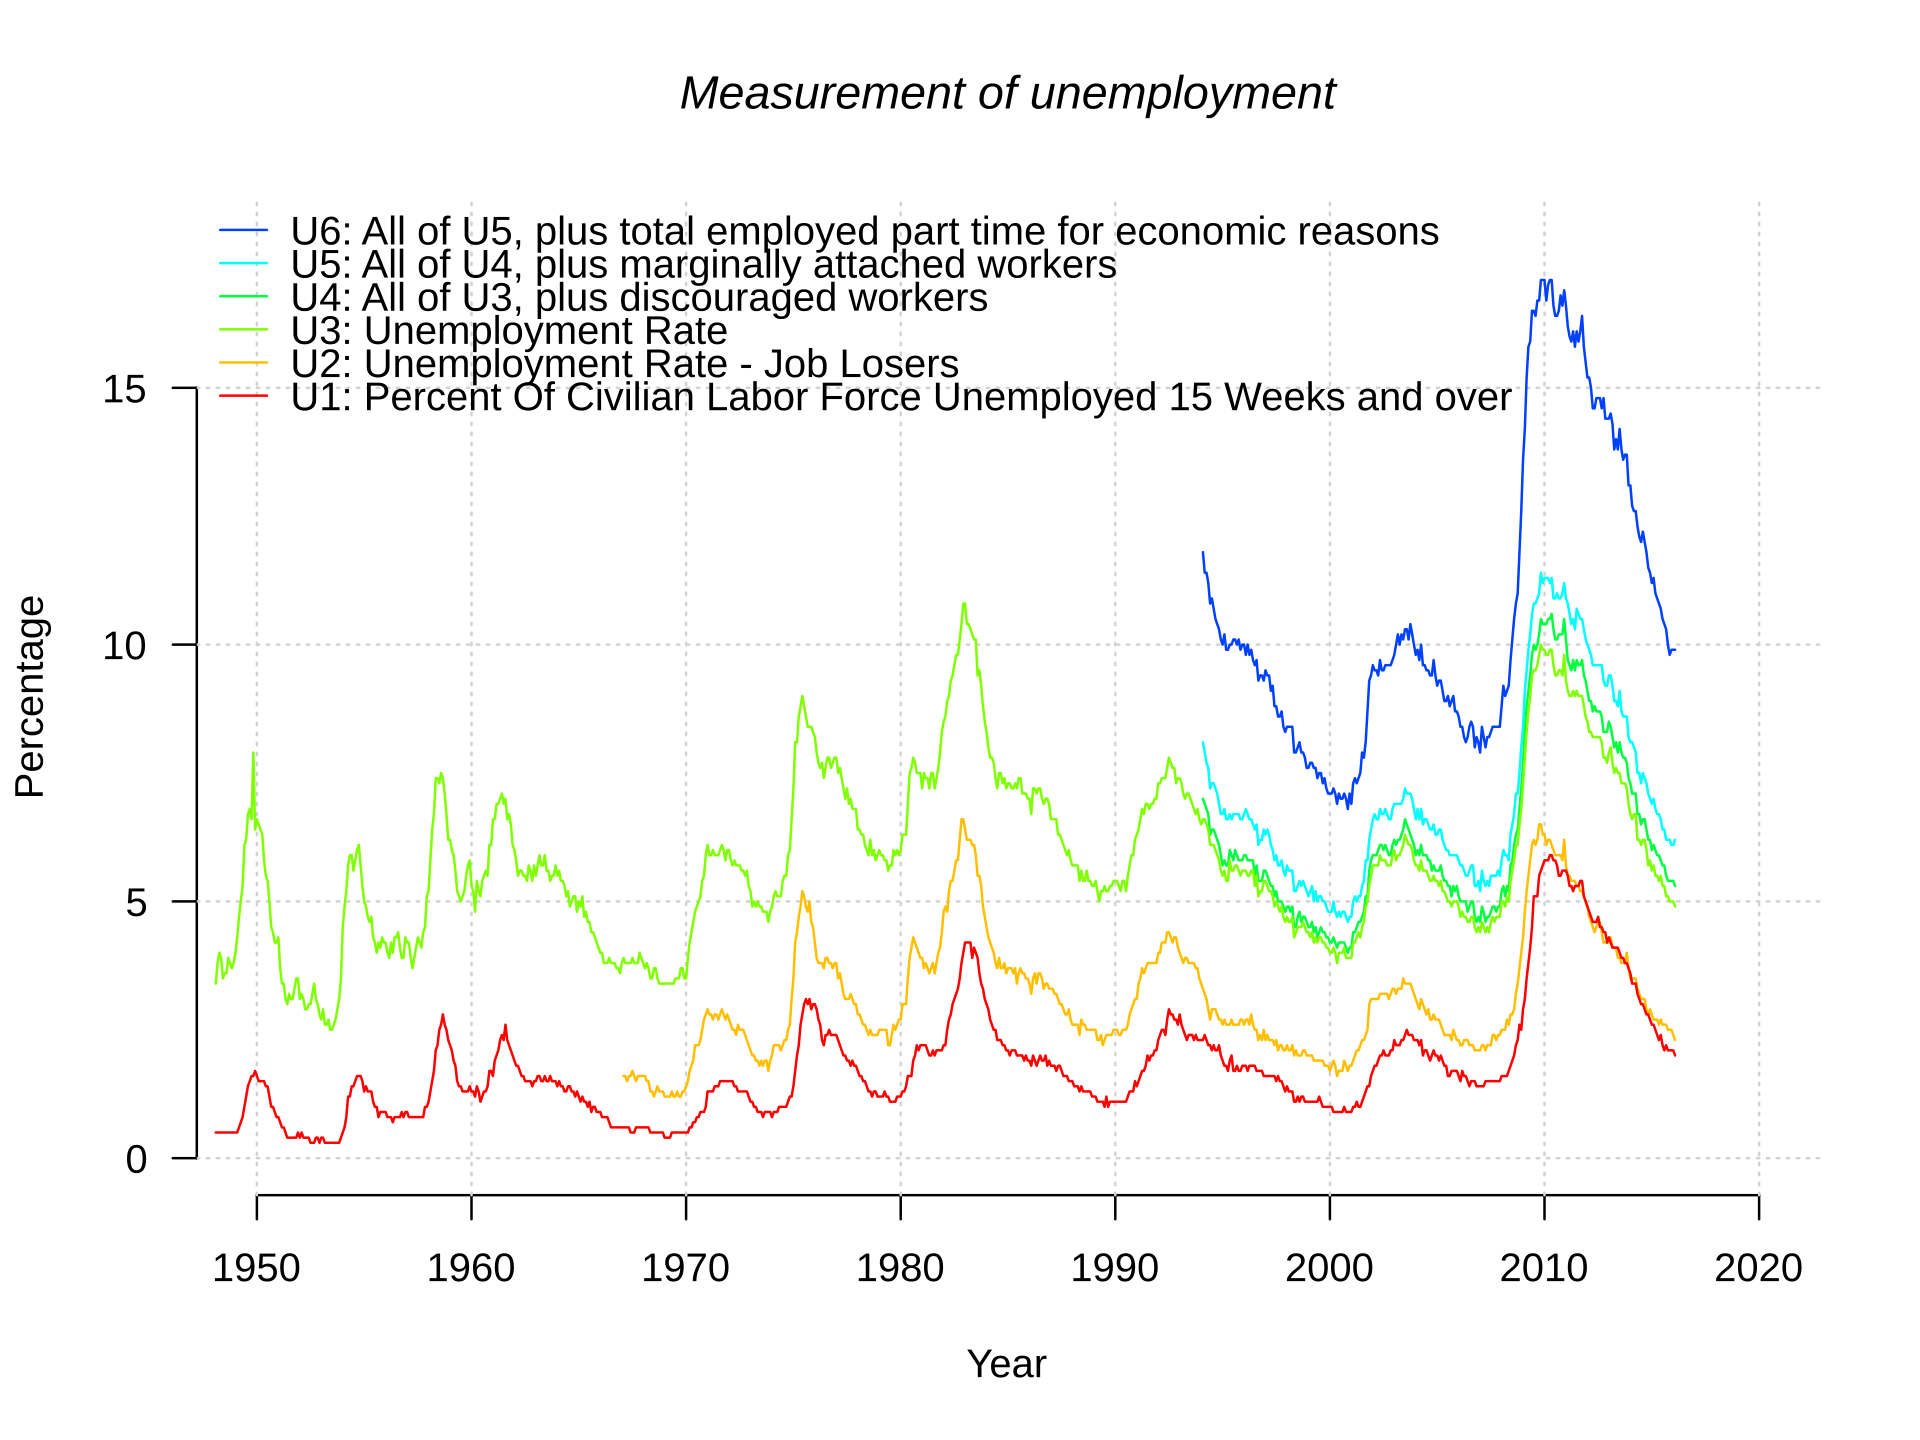
\includegraphics[scale=0.15]{unemployment_2.png}
\end{center}

\end{frame}

%@@@@@@@@@@@@@@@@@@@@@@@@@@@@@@@@@@@@@@@@@@@@@@@@@
\begin{frame}
\frametitle{Choices}

\begin{itemize}
\item How many public water systems are there in the US?
\bigskip
\bigskip
\item Public water system: $\geq$15 service connections or service to an average of $\geq$ 25 people for $\geq$ 60 days a year;
\bigskip
\bigskip
\item With this definition, over 148k;
\begin{itemize}
\item Community Water System;
\item Non-Transient Non-Community Water System;
\item Transient Non-Community Water System.
\end{itemize}
\end{itemize}

\end{frame}



%@@@@@@@@@@@@@@@@@@@@@@@@@@@@@@@@@@@@@@@@@@@@@@@@@
\begin{frame}
\frametitle{Choices}
\begin{itemize}
\item ``As answers to policy problems, the resolution numbers offer is nothing more than a human decision about how to count as"  (i.e. numbers $=$ metaphors);
\bigskip
\bigskip
\item Wrongful exclusion:
\begin{itemize}
\item Assertion of a likeness where measurement assigns a difference;
\item Examples: unemployed, homelessness, grades, excess mortality during war;
\end{itemize}
\bigskip
\bigskip
\item Wrongful inclusion:
\begin{itemize}
\item Assertion of a difference where measurement assigns a likeness;
\item Example: excess mortality during war (Iraq war deaths);
\end{itemize}
\end{itemize}
\end{frame}

%%@@@@@@@@@@@@@@@@@@@@@@@@@@@@@@@@@@@@@@@@@@@@@@@@@
%\begin{frame}
%\frametitle{Hidden messages in using numbers}
%\begin{itemize}
%\item Expertise and authority (e.g. Mitt Romney);
%\bigskip
%\bigskip
%\item Recognition or assertion that something is widespread but unobserved (e.g. COVID);
%\bigskip
%\bigskip
%\item Claim of clear boundaries (e.g. insurgency);
%\bigskip
%\bigskip
%\item Creation of community (e.g. population);
%\bigskip
%\bigskip
%\item Bargaining (e.g. breaking down a problem like Roe v Wade).
%\end{itemize}
%\end{frame}

%@@@@@@@@@@@@@@@@@@@@@@@@@@@@@@@@@@@@@@@@@@@@@@@@@
\begin{frame}
\frametitle{Artifacts and dangers...}
\begin{columns}
\begin{column}{0.5\textwidth}

\begin{itemize}
\item Numbers can reduce conflicts to a single dimension;
\begin{itemize}
\item e.g., if we only considered the energy density of fuel sources (versus cost or safety), we might draft policy to build more nuclear power plants...
\end{itemize} 
\item Numbers legitimize political decisions;
\begin{itemize}
\item ...and sometimes mask the political nature of a decision;
\item For example, numbers suggest that safety can be defined though science (but recall the complexity and subjective nature of ``Security");
\item Back to Egan: What is a ``safe number of organisms that could be discharged per cubic meter of water?"
\end{itemize}
\end{itemize}

\end{column}
\begin{column}{0.5\textwidth}
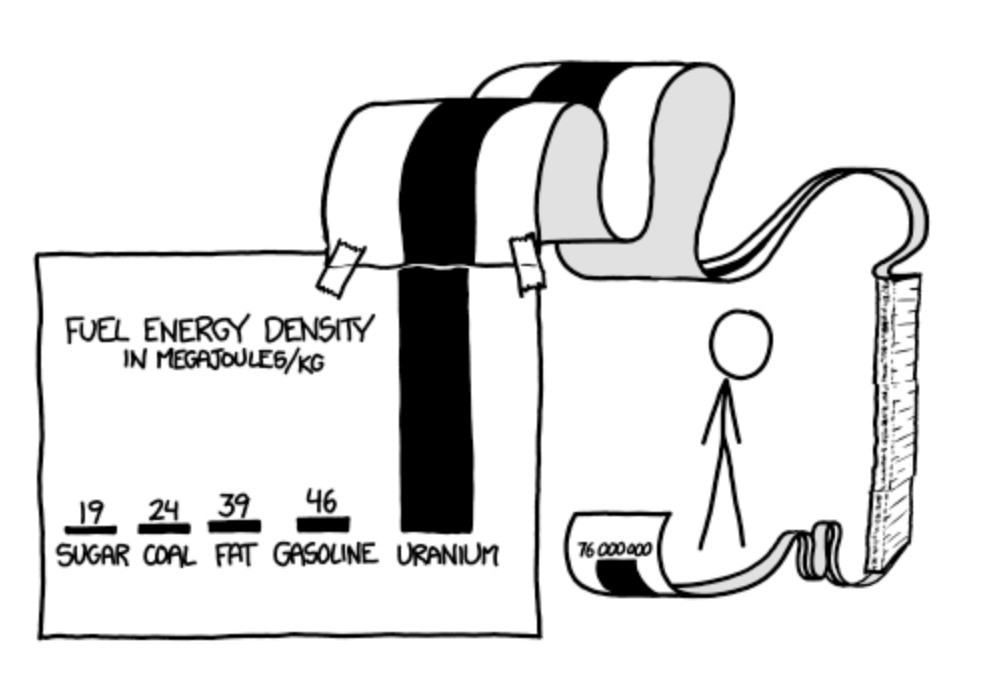
\includegraphics[scale=0.4]{energy.png}
\end{column}
\end{columns}

\end{frame}

%@@@@@@@@@@@@@@@@@@@@@@@@@@@@@@@@@@@@@@@@@@@@@@@@@
\begin{frame}
\frametitle{Artifacts and dangers...}
\begin{columns}
\begin{column}{0.5\textwidth}

\begin{itemize}
\item Numbers can reduce conflicts to a single dimension;
\begin{itemize}
\item e.g., if we only considered the energy density of fuel sources (versus cost or safety), we might draft policy to build more nuclear power plants...
\end{itemize}
\item Numbers legitimize political decisions;
\begin{itemize}
\item ...and sometimes mask the political nature of a decision;
\item For example, numbers suggest that safety can be defined though science (but recall the complexity and subjective nature of ``Security");
\item Back to Egan: What is a ``safe number of organisms that could be discharged per cubic meter of water?"
\end{itemize}
\end{itemize}

\end{column}
\begin{column}{0.5\textwidth}
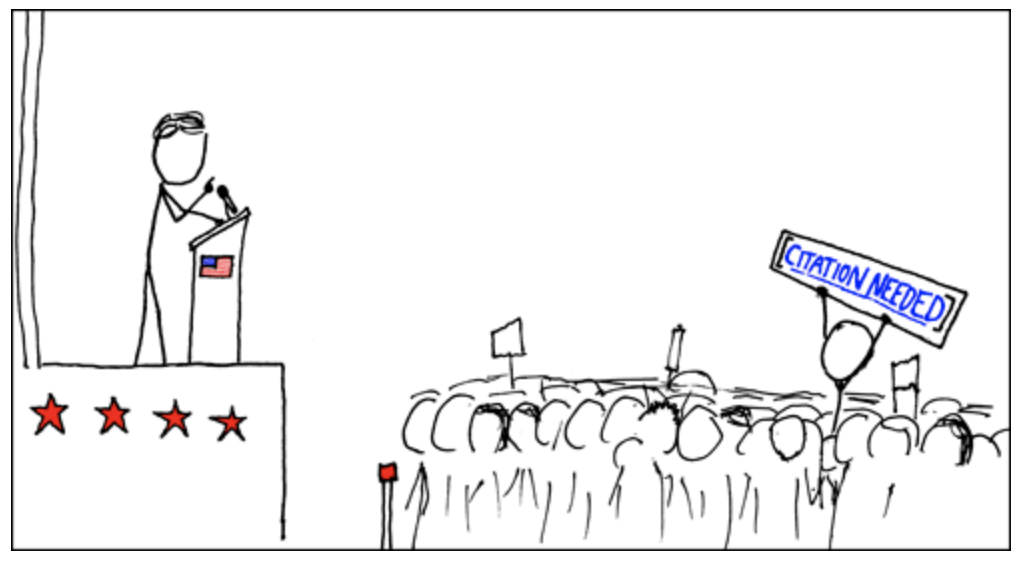
\includegraphics[scale=0.4]{speech.png}
\end{column}
\end{columns}

\end{frame}

%@@@@@@@@@@@@@@@@@@@@@@@@@@@@@@@@@@@@@@@@@@@@@@@@@
\begin{frame}
\frametitle{Observer Effects}
\begin{itemize}
\item In science (especially social science), we confront observer effects–the fact that things, and especially people, behave differently when observed;
\begin{itemize}
\item Physics: uncertainty (Heisenberg) and it's generalizations;
\item Social science: poll responses;
\end{itemize}
\bigskip
\item Can interact with counting -- by counting people as part of a group, a policy may induce them to act as a group (statistical community becomes a natural community). Group theories of politics (e.g., pluralism) tell us to expect these groups to then advocate for resources, privileges, or protection in future policy processes.
\bigskip
\item Question: if the Department of Justice Antitrust Division measures market concentration to decide whether to permit corporate mergers and acquisitions, how do you think this might affect how large companies lobby regarding the definition of their ``market"?
\end{itemize}
\end{frame}

%@@@@@@@@@@@@@@@@@@@@@@@@@@@@@@@@@@@@@@@@@@@@@@@@@
\begin{frame}

\begin{center}
\Huge\textbf{Why should we care?}\\
\bigskip
\bigskip
\large The power to measure is the power to control.  Measurers have a lot of discretion in their choice of what and how to measure.\\
\end{center}

\end{frame}

%@@@@@@@@@@@@@@@@@@@@@@@@@@@@@@@@@@@@@@@@@@@@@@@@@
\begin{frame}

\begin{center}
\Huge\textbf{Problems : Causes}\\
\bigskip
\bigskip
\large How the world works
\end{center}

\end{frame}

%@@@@@@@@@@@@@@@@@@@@@@@@@@@@@@@@@@@@@@@@@@@@@@@@@
\begin{frame}
\frametitle{To Know the Causes of Things}
\begin{itemize}
\item \textbf{Causality}: necessary and sufficient conditions;
\begin{itemize}
\item Very difficult;
\item Absolutely crucial for effective problem solving;
\end{itemize}
\bigskip
\bigskip
\item Ideal: causes are objective and can be identified by scientific analysis;
\bigskip
\bigskip
\item Stone: causal analysis has prescriptive power:
\begin{itemize}
\item Like numbers, causes highlight some aspects of a problem and ignore others;
\item Causal chains are stories that define problems and assign blame;
\item Because they have this power there are incentives to use them strategically.
\end{itemize}
\end{itemize}
\end{frame}

%@@@@@@@@@@@@@@@@@@@@@@@@@@@@@@@@@@@@@@@@@@@@@@@@@
\begin{frame}
\frametitle{Typology of causal theories (Table 9.1)}
\begin{itemize}
\item Unguided actions/Intended consequences -- \textbf{mechanical cause}:
\begin{itemize}
\item Machines that perform to spec but cause harm;
\item Rigid bureaucratic routines;
\end{itemize}
\bigskip
\item Unguided actions/unintended consequences -- \textbf{accidental cause}:
\begin{itemize}
\item Natural disasters;
\item Fate/bad luck;
\end{itemize}
\bigskip
\item Guided actions/Intended consequences -- \textbf{intentional cause}:
\begin{itemize}
\item Oppression;
\item Conspiracy;
\item Known but ignored harms;
\item Victim blaming;
\end{itemize}
\bigskip
\item Guided actions/unintended consequences -- \textbf{inadvertent cause}:
\begin{itemize}
\item unintended side effects;
\item Victim blaming.
\end{itemize}
\end{itemize}
\end{frame}

%@@@@@@@@@@@@@@@@@@@@@@@@@@@@@@@@@@@@@@@@@@@@@@@@@
\begin{frame}
\frametitle{Complexity}
\begin{itemize}
\item Many policy problems--such as toxic hazards, global warming, oil spills, and food safety--require a more \textbf{complex model of cause}... can shift problems to appear accidental or unintended;
\bigskip
\item Complex systems:
\begin{itemize}
\item Social systems necessary to solve modern problems are inherently complex;
\item Multiple actors $+$ complex feedback loops $=$ certain but impossible to anticipate failure;
\end{itemize}
\bigskip
\item Institutional complexity:
\begin{itemize}
\item Social problems caused by webs of large organizations with built-in incentive structures and patterns of behavior;
\item e.g. US government procurement;
\end{itemize}
\bigskip
\item Historical complexity:
\begin{itemize}
\item Decisions in one period determine the choices available in future periods;
\item Path dependence -- e.g. QWERTY keyboards.
\end{itemize}
\end{itemize}
\end{frame}

%%@@@@@@@@@@@@@@@@@@@@@@@@@@@@@@@@@@@@@@@@@@@@@@@@@
%\begin{frame}
%\frametitle{The banality of evil}
%\begin{itemize}
%\item These questions of intentionality and complexity are essential to the concept of accountability;
%\bigskip
%\bigskip
%\item ``I was just following orders" $\sim$ Adolf Eichmann;
%\begin{itemize}
%\item If Eichmann’s work, as a bureaucrat, is seen as a mechanical process of following orders or as embedded in a complex system, then he is not a policy actor and thus not responsible;
%\item If seen as an intentional architect, then he is a policy actor and thus entirely responsible;
%\end{itemize}
%\bigskip
%\bigskip
%\item Not just for the Holocaust -- the podcast, Death by a Thousand Cuts applied philosopher Hannah Arendt’s concept of “the Banality of Evil” to agency decisions;
%\bigskip
%\bigskip
%\item How might we draw lines between people who are simply following orders and thus blameless and those who act consciously, and are thus responsible?
%\end{itemize}
%\end{frame}

%%@@@@@@@@@@@@@@@@@@@@@@@@@@@@@@@@@@@@@@@@@@@@@@@@@
%\begin{frame}
%\frametitle{Legitimacy}
%\begin{itemize}
%\item Science: arbiter of empirical questions;
%\bigskip
%\bigskip
%\item Law: hears claims, examines evidence, pronounces judgments;
%\bigskip
%\bigskip
%\item This is why good research and understanding of legal authority are so important for writing policy memos. Without evidence and authority that your audience sees as legitimate, they will not take your recommendations seriously.
%\end{itemize}
%\end{frame}

%@@@@@@@@@@@@@@@@@@@@@@@@@@@@@@@@@@@@@@@@@@@@@@@@@
\begin{frame}

\begin{center}
\Huge\textbf{Why should we care?}\\
\bigskip
\bigskip
\large The role of causality is why good research and understanding of legal authority are so important for writing policy memos. Without evidence and authority that your audience sees as legitimate, they will not take your recommendations seriously.\\
\bigskip
Causal theories are efforts to control interpretations and images of problems, to describe harms and difficulties, to attribute them to actions of actors, and thereby to allocate government power to stop the harm.
\\
\end{center}

\end{frame}


\end{document}






